\documentclass[11pt,a4paper]{article}
% \documentclass[a4paper]{article}
% \usepackage[brazil]{babel} % carrega portugues brasileiro
\usepackage[utf8]{inputenc}
\usepackage[T1]{fontenc}
\usepackage[top=2cm, bottom=2cm, left=2cm, right=2cm]{geometry} %margens menores!
\usepackage{graphicx} % incluir figuras .eps
\usepackage{tabularx}
\usepackage{color} % colorir texto
\usepackage{indentfirst}
\usepackage{textcomp}
\usepackage[colorlinks=true]{hyperref}
\usepackage{amssymb,amsmath}
\usepackage{float}
\usepackage{wrapfig}
\usepackage[skip=2pt]{caption} % example skip set to 2pt

% \usepackage{siunitx}
% \usepackage[ampersand]{easylist}

\title{HERMES System Installation Guide}


\author{
       \large
       \mbox{Rhizomatica} \\
       \mbox{}\\ 
       \textsc{Rafael Diniz}
        rafael@rhizomatica.org\\
%        \normalsize
%        we want the airwaves
%        \texttt{Brasília - Brasil}\\
}
\date{\today}

\begin{document}

\maketitle

\begin{figure*}[!ht]

\includegraphics[width=1\textwidth]{pictures/logoh.png}
\end{figure*}

\begin{abstract}

  High-Frequency Emergency and Rural Multimedia Exchange System (HERMES) installation procedure for the sBitx v2 radio.

\end{abstract}

% \newpage

\tableofcontents

\setlength{\parindent}{0em}
\setlength{\parskip}{1em}

\section{Introduction}

This guide goes through the steps needed for HERMES system installation.

%\begin{figure*}[!ht]
%
\includegraphics[width=1\textwidth]{pictures/hermes.png}
%\end{figure*}

\section{Power supply and consumption}

In order to connect the radio to the power source, a power cable is provided. One side of the
cable comes with a XT60 connector (Figure~\ref{fig:psu2}) and connects to the radio, and the other end is bare ended,
and should be connected to the positive (Red) and negative (Black) of a 12V battery system, or power
supply. Power consumption is not more than 1.5 A in receive mode, and 9 A in transmit mode.

\begin{figure}[!ht]
  \centering
  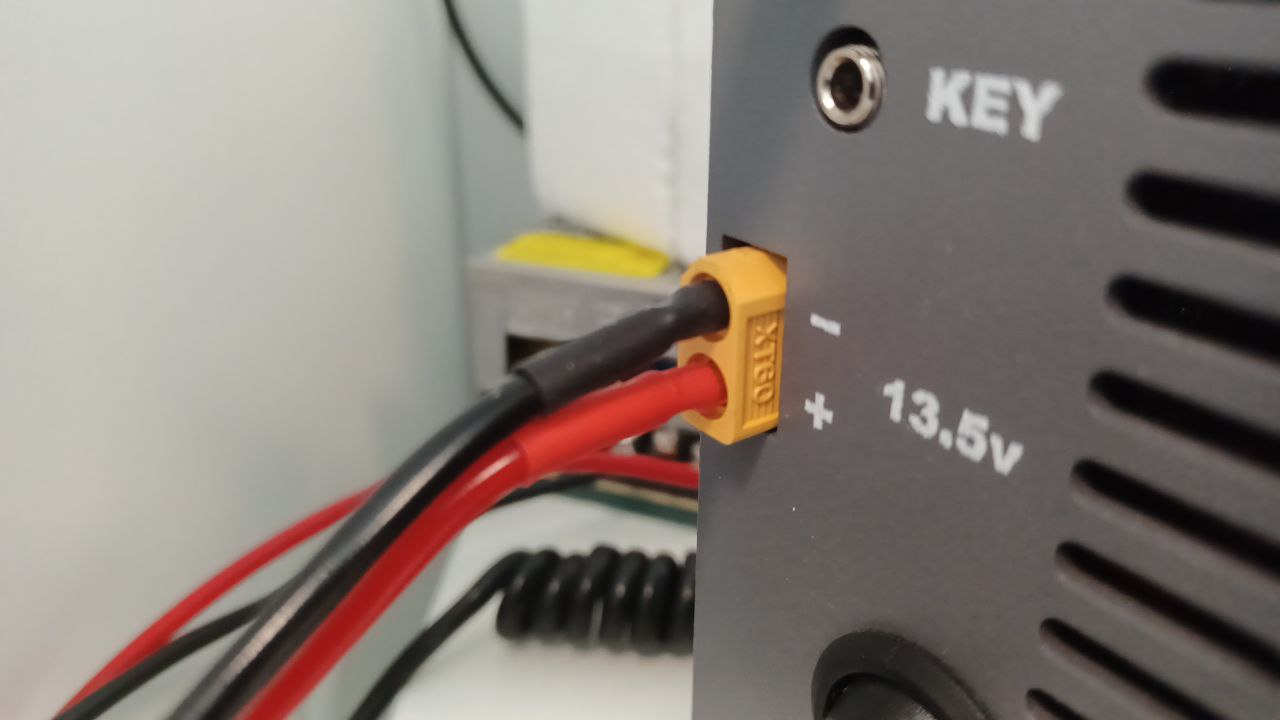
\includegraphics[width=0.5\textwidth]{pictures/psu1.jpeg}
  \caption{The radio-side of the power cables where the XT60 connector is located.}
  \label{fig:psu1}
\end{figure}

\begin{figure}[!ht]
  \centering
  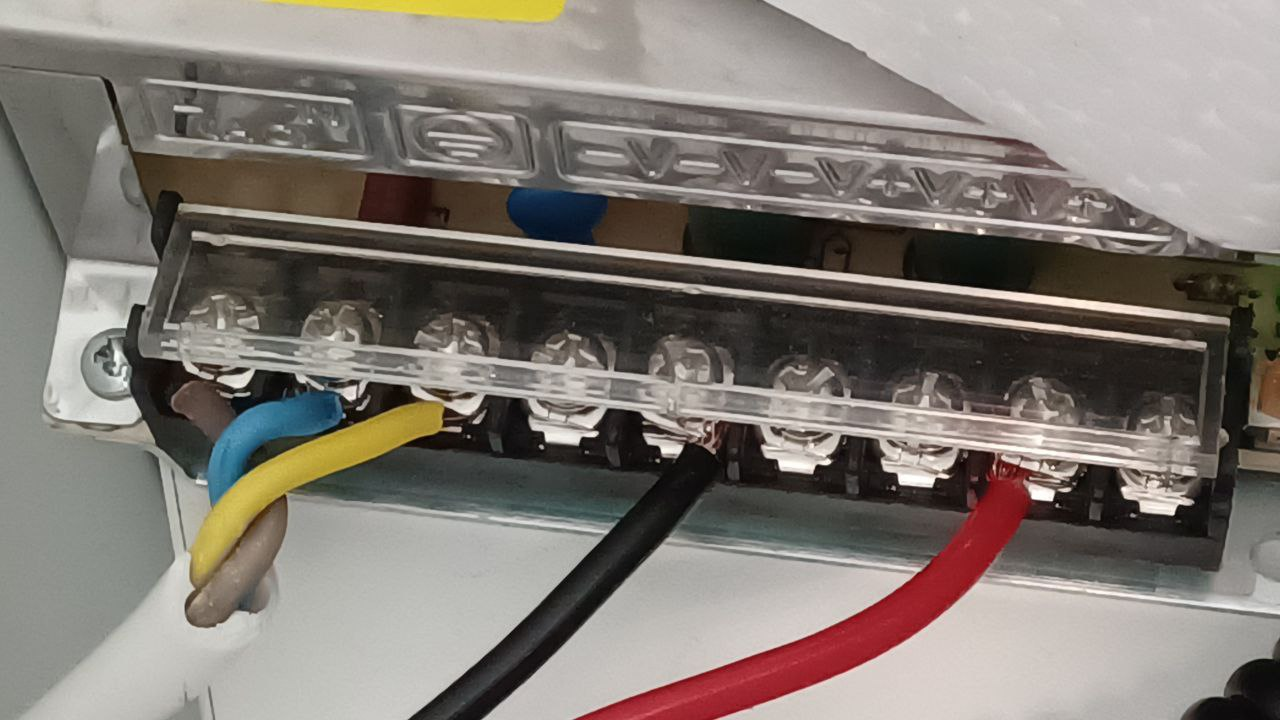
\includegraphics[width=0.5\textwidth]{pictures/psu2.jpeg}
  \caption{Red (+) and black (-) cables connected to appropriate power supply terminals.}
  \label{fig:psu2}
\end{figure}


\section{Initial setup to allow boot from USB pendrive}

This step is needed in order to enable the HERMES installer to run from a USB pendrive.

First connect a USB keyboard to the radio, and then connect the radio to the network (RJ45) cable with appropriate Internet connection.
Then click in the Terminal icon shown in Figure~\ref{fig:terminal}.

\begin{figure}[!ht]
  \centering
  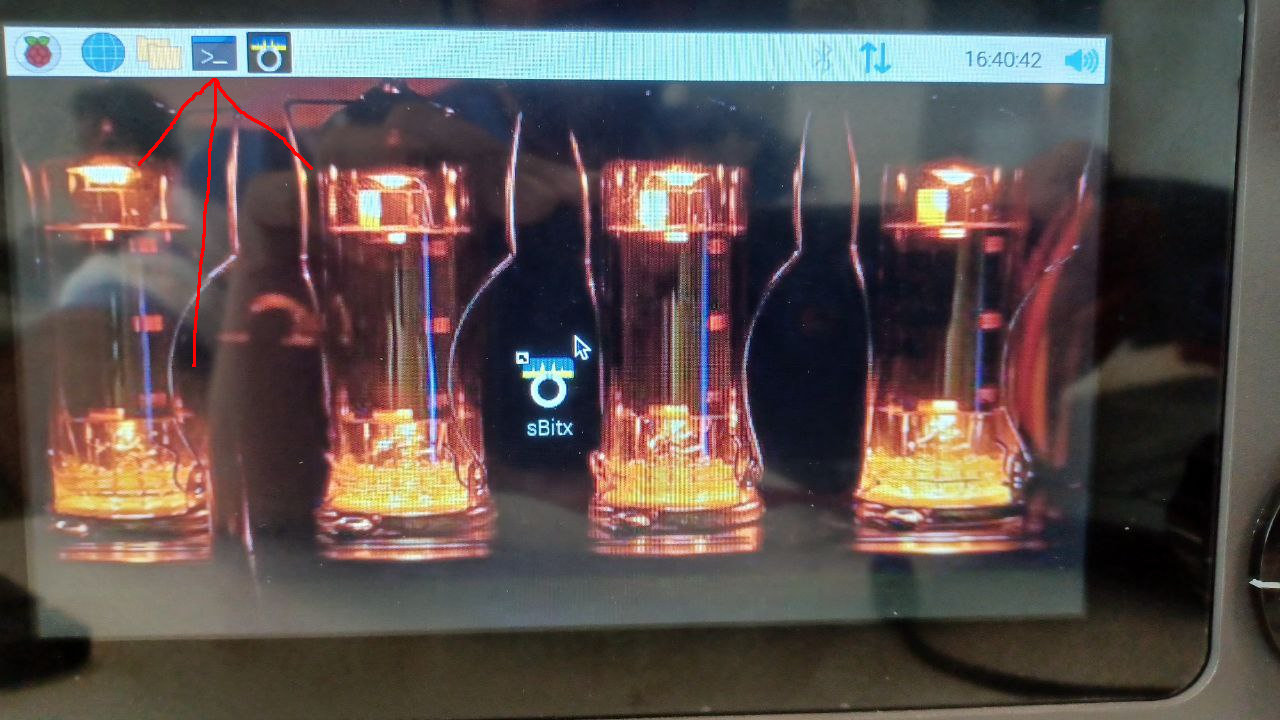
\includegraphics[width=0.5\textwidth]{pictures/screen1-edited.jpeg}
  \caption{Screen of the radio and the ``Terminal'' icon pointed by a red arrow.}
  \label{fig:terminal}
\end{figure}

After opening the terminal window, type:

\begin{itemize}
\item sudo su
\item apt-get update
\item apt-get install rpi-eeprom
\item raspi-config
\end{itemize}

At this point the screen shown in Figure~\ref{fig:screen3} should appear.

\begin{figure}[!ht]
  \centering
  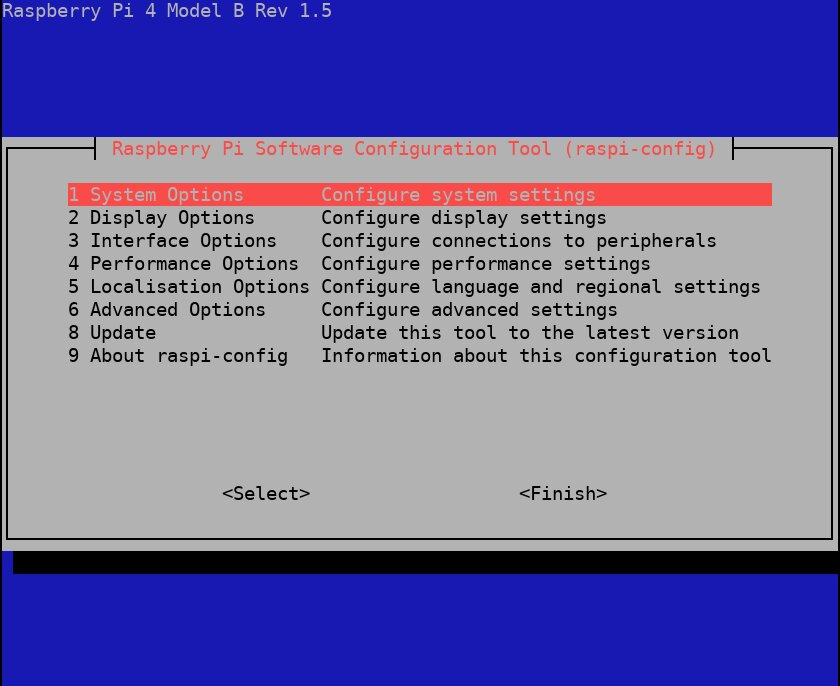
\includegraphics[width=0.5\textwidth]{pictures/screen3.jpg}
  \caption{Configuration software screen (raspi-config tool).}
  \label{fig:screen3}
\end{figure}

Choose the options of the menu in the following order using the keyboard arrow and Tab keys (as shows in Figures):
\begin{itemize}
\item Step 1: Option 6 (Advanced Options)
\item Step 2: Option A6 (Boot Order)
\item Step 3: Option B2 (USB Boot)
\item Step 4: Finish
\end{itemize}

\begin{figure}[H]
  \centering
  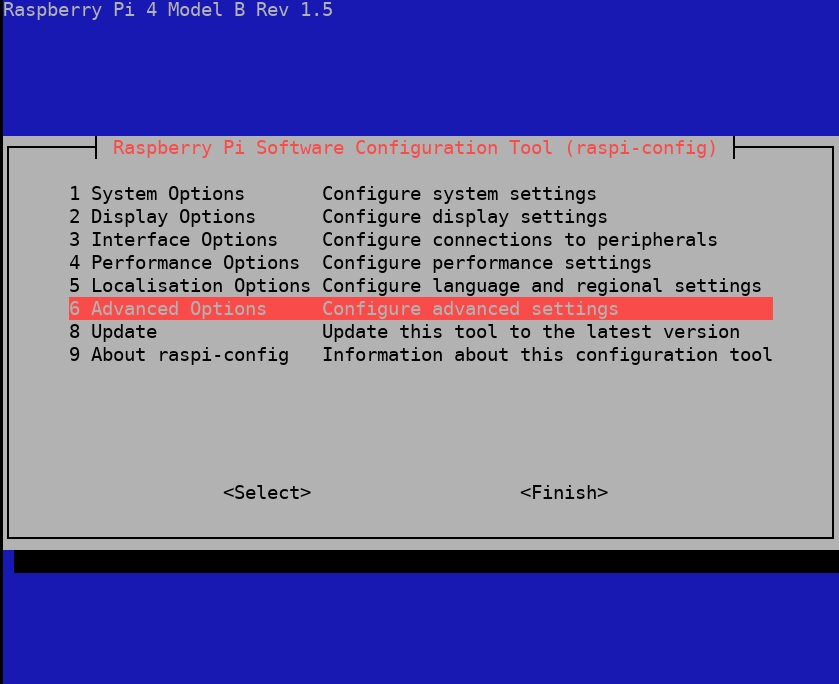
\includegraphics[width=0.5\textwidth]{pictures/screen4.jpg}
  \caption{Menu option to select (step 1).}
  \label{fig:screen4}
\end{figure}

\begin{figure}[H]
  \centering
  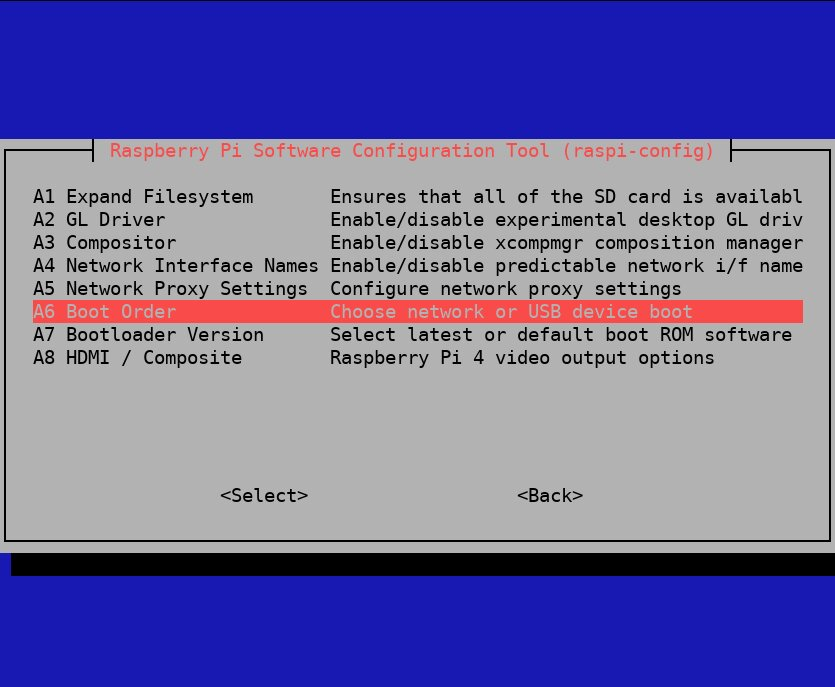
\includegraphics[width=0.5\textwidth]{pictures/screen5.jpg}
  \caption{Menu option to select (step 2).}
  \label{fig:screen5}
\end{figure}

\begin{figure}[H]
  \centering
  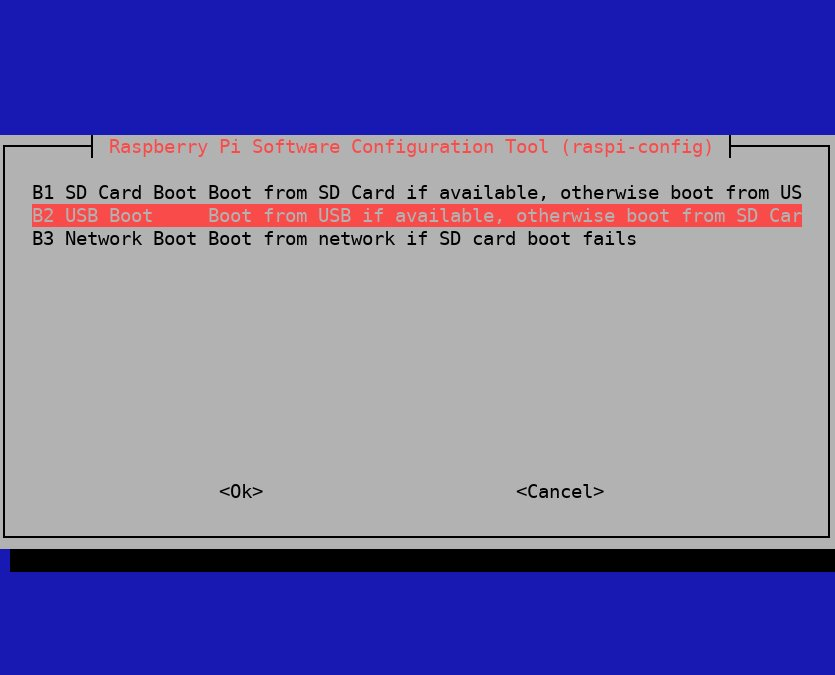
\includegraphics[width=0.5\textwidth]{pictures/screen6.jpg}
  \caption{Menu option to select (step 3).}
  \label{fig:screen6}
\end{figure}

Then just accept the option to reboot the radio.
Now the radio is ready to run the HERMES installer. If needed, in order to turn off the radio, type the following in the terminal window (just after raspi-config):

\begin{itemize}
\item halt
\end{itemize}

And after some seconds, when the screen goes black, turn off the radio (using the power key below the power socket).

\section{HERMES USB installer preparation}

A USB pendrive of at least 8 GB is needed. A computer is needed to prepare the USB pendrive.

The installer should be downloaded from: \url{https://aco-connexion.org/downloads/installer-image.img.zip}.

After the download is finished, the file should be ``unzipped'', as shown in Figures \ref{fig:extract1}, \ref{fig:extract2}
and \ref{fig:extract3}.
The extracted file should have the name: ``installer-image.img''.

\begin{figure}[H]
  \centering
  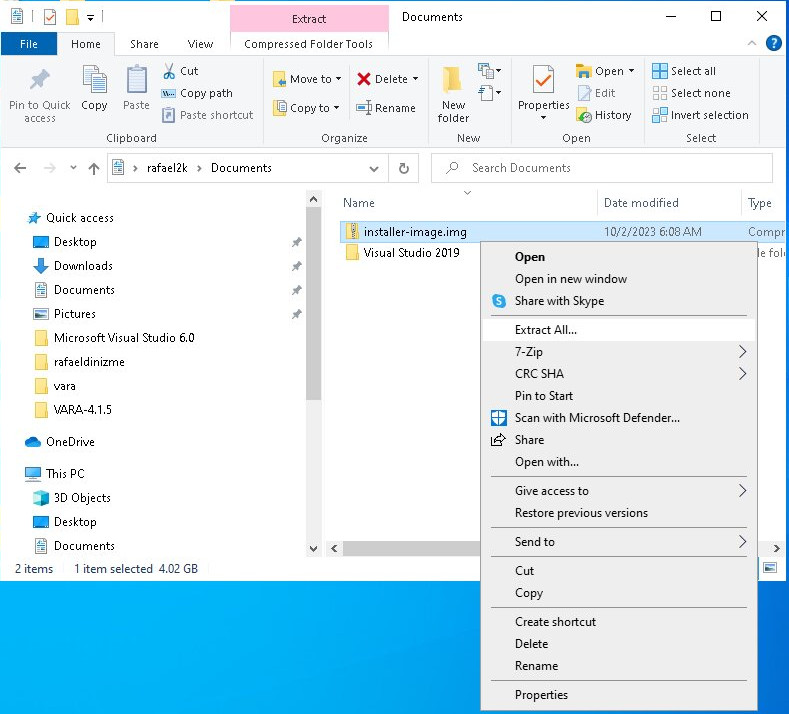
\includegraphics[width=0.6\textwidth]{pictures/extract-1-ed.jpg}
  \caption{Unzipping the installer file.}
  \label{fig:extract1}
\end{figure}

\begin{figure}[H]
  \centering
  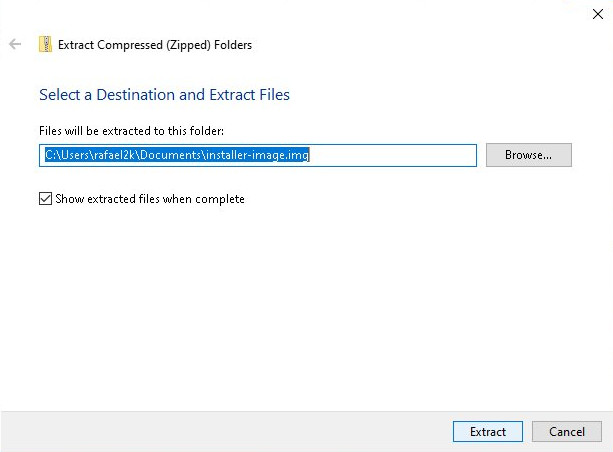
\includegraphics[width=0.6\textwidth]{pictures/extract-2-ed.jpg}
  \caption{Setting the installer file name.}
  \label{fig:extract2}
\end{figure}

\begin{figure}[H]
  \centering
  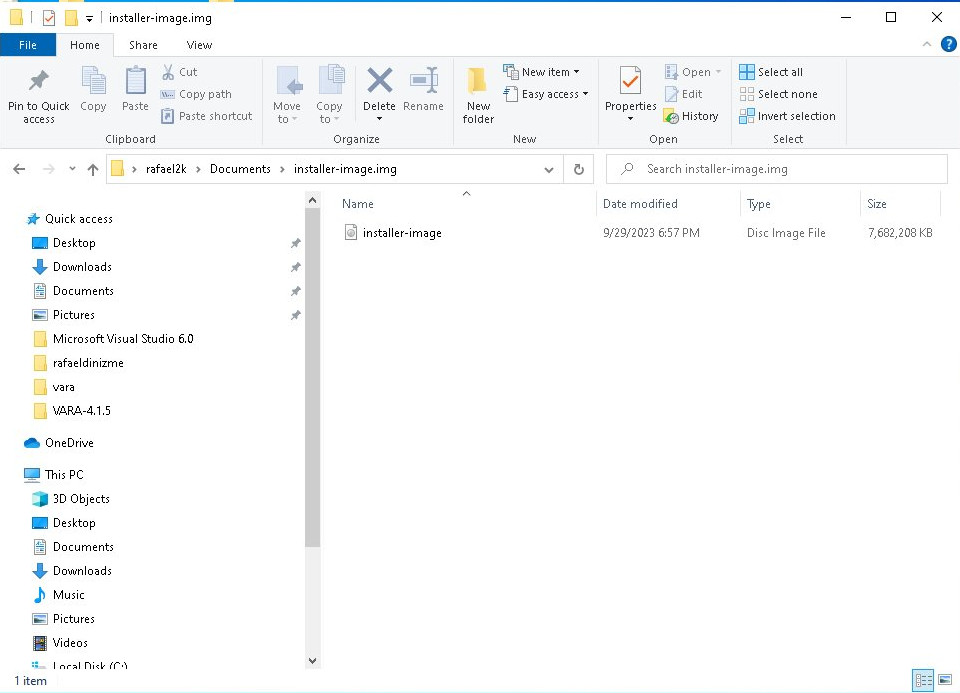
\includegraphics[width=0.6\textwidth]{pictures/extract-3-ed.jpg}
  \caption{Installer file after unzip.}
  \label{fig:extract3}
\end{figure}

Then, for copying the installer to the USB pendrive, use the following software (or other raw image writer or flasher), called
Etcher (supported on Windows, MacOS and Linux), available in \url{https://etcher.balena.io/}. The download is available on this website,
as shown in Figure \ref{fig:balena1} (eg: for Windows choose the first option).

\begin{figure}[H]
  \centering
  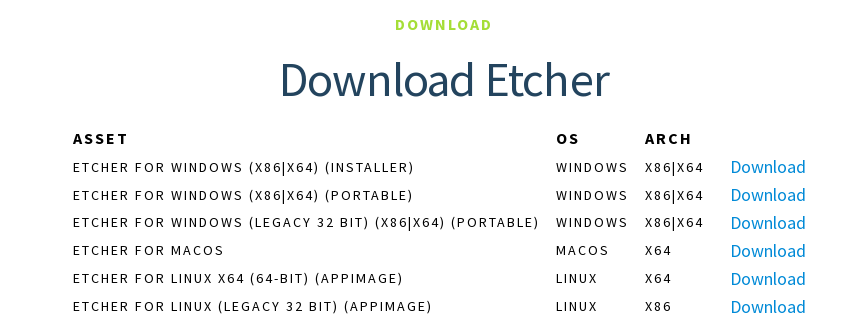
\includegraphics[width=0.6\textwidth]{pictures/balena-1.png}
  \caption{Download options for Etcher software.}
  \label{fig:balena1}
\end{figure}

Run the software Etcher, choose the option ``Flash from file'' and select the file ``installer-image.img'', as shown in Figures \ref{fig:balena2}, \ref{fig:balena3} and \ref{fig:balena4}.

\begin{figure}[H]
  \centering
  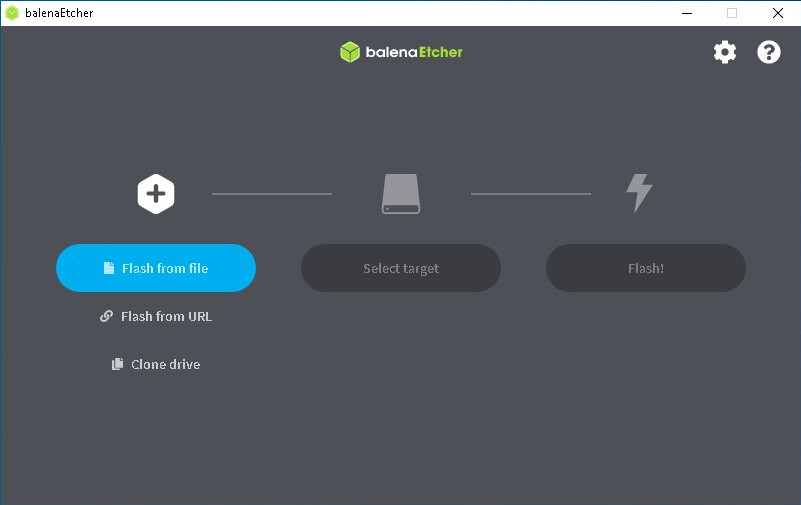
\includegraphics[width=0.6\textwidth]{pictures/balena-2-ed.jpg}
  \caption{First screen of Etcher, ``Flash from file'' selected.}
  \label{fig:balena2}
\end{figure}

\begin{figure}[H]
  \centering
  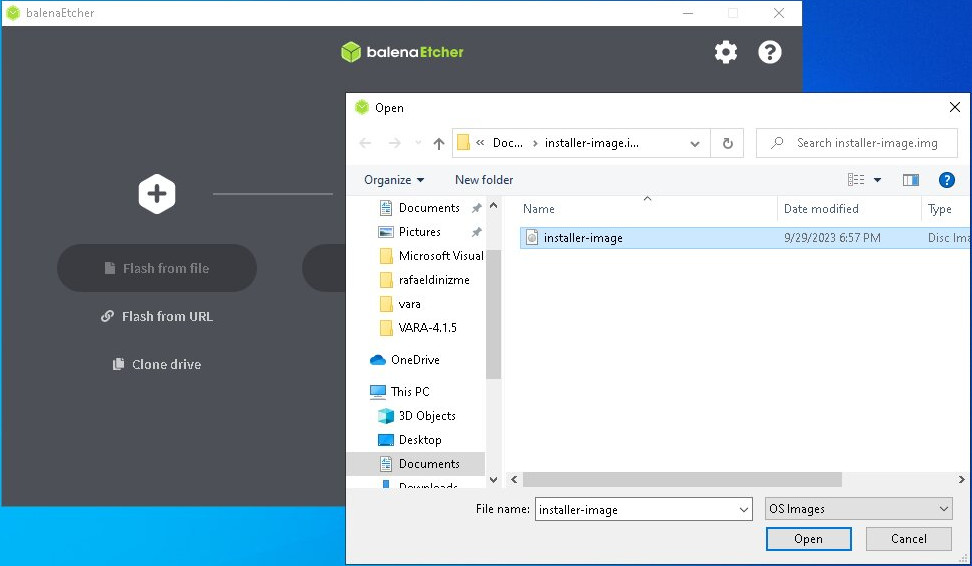
\includegraphics[width=0.6\textwidth]{pictures/balena-3-ed.jpg}
  \caption{Choose the file ``installer-image''.}
  \label{fig:balena3}
\end{figure}

\begin{figure}[H]
  \centering
  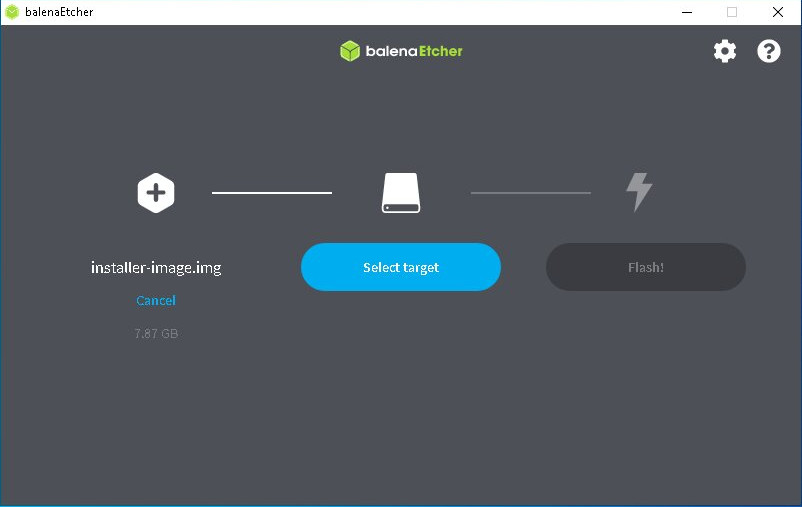
\includegraphics[width=0.6\textwidth]{pictures/balena-4-ed.jpg}
  \caption{Select the USB pendrive to be used as installer.}
  \label{fig:balena4}
\end{figure}

After the copy is finished, insert the USB pendrive with the HERMES installer in the radio, as shown in Figure~\ref{fig:pen1}.
Make sure the radio is turned OFF before inserting the USB pendrive.


\begin{figure}[H]
  \centering
  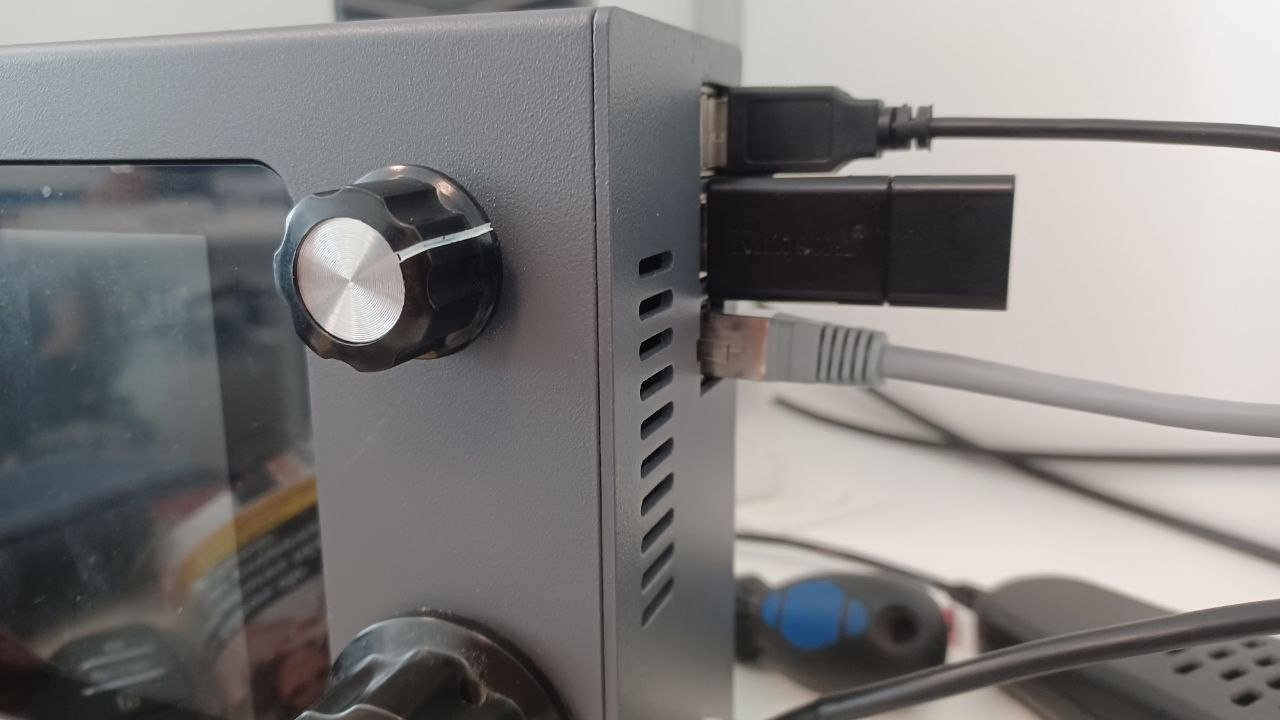
\includegraphics[width=0.5\textwidth]{pictures/usb-1.jpeg}
  \caption{Radio with USB pendrive connected, together with keyboard and network cable.}
  \label{fig:pen1}
\end{figure}


\section{HERMES installation}

The HERMES installation procedure will set up the sBitx v2 radio with HERMES system,
and perform the station-specific setup.

The installation is done in two steps. The first one with the
pendrive inserted in the radio, and the second without the pendrive.

After preparing the USB pendrive and plugging it to the radio, turn on the radio.

When asked if you want to proceed with the installation, answer ``y'' and press ENTER, as shown in Figure~\ref{fig:inst1}.

\begin{figure}[H]
  \centering
  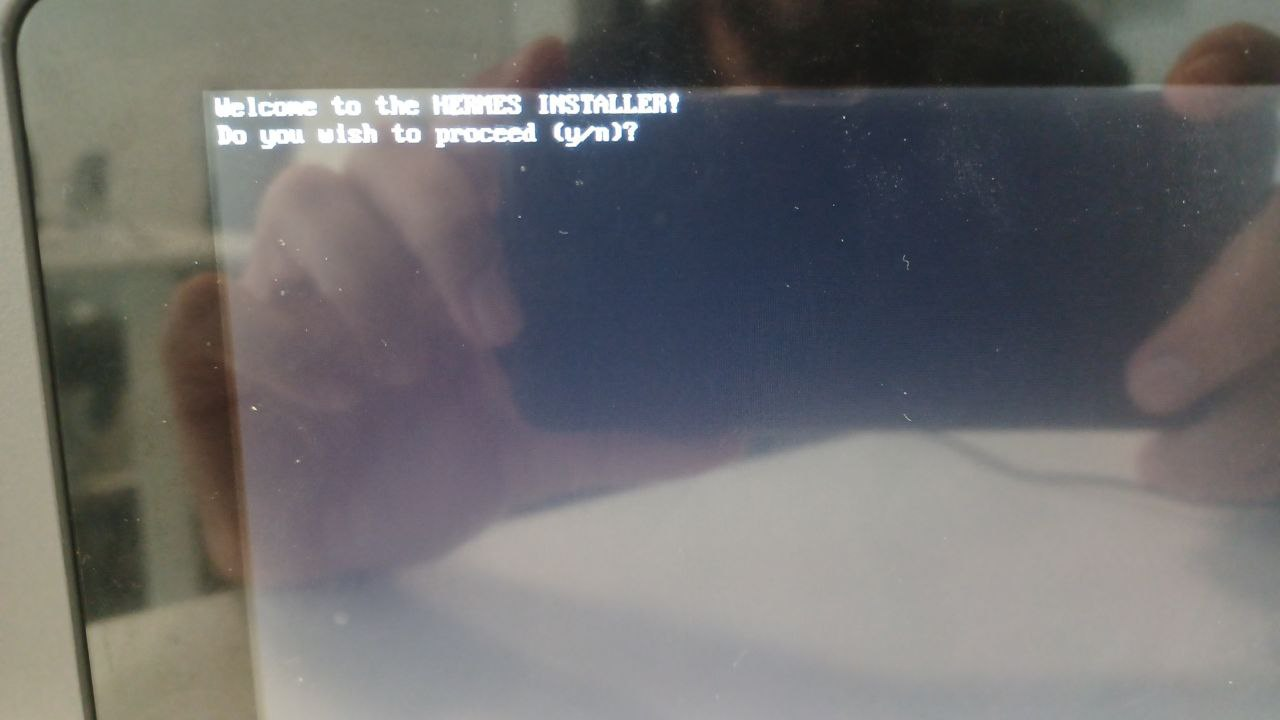
\includegraphics[width=0.5\textwidth]{pictures/inst-1.jpg}
  \caption{HERMES interactive installer starting.}
  \label{fig:inst1}
\end{figure}

When asked if you want to write HERMES (copy the system), anwser ``y'' and press ENTER, as shown in Figure~\ref{fig:inst2}.

\begin{figure}[H]
  \centering
  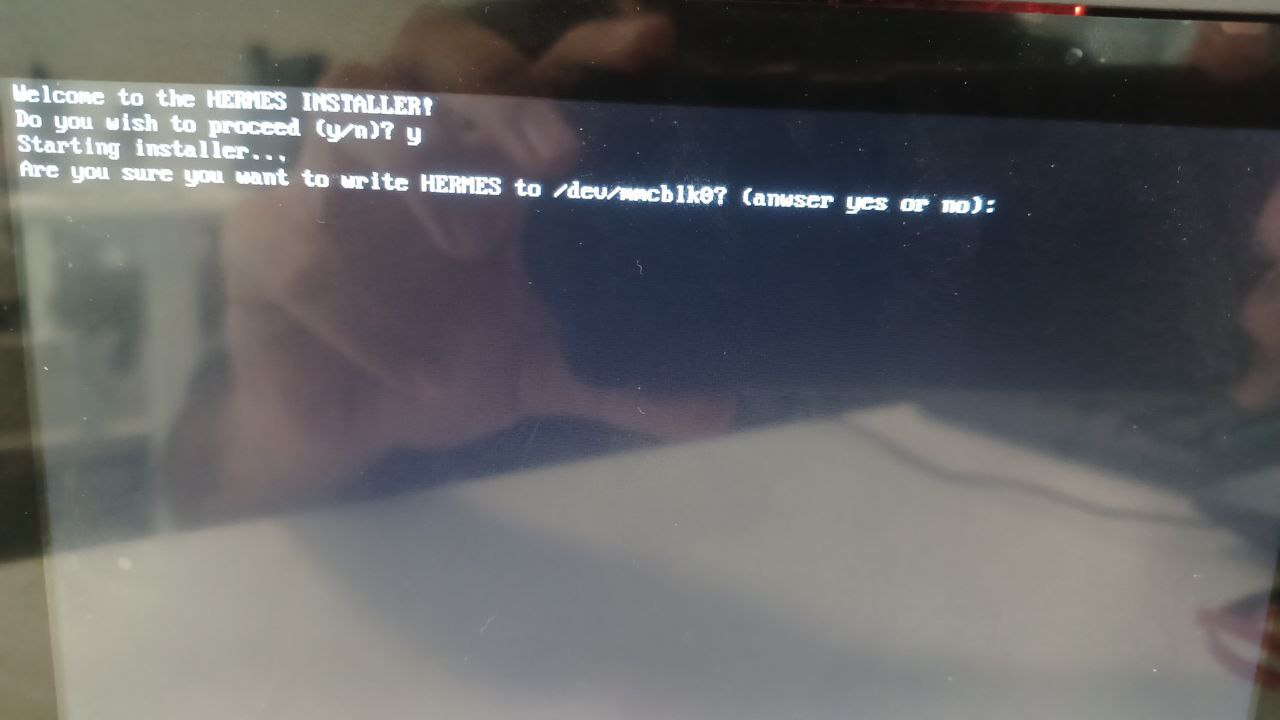
\includegraphics[width=0.5\textwidth]{pictures/inst-2.jpg}
  \caption{HERMES installer question to start writing to internal radio memory.}
  \label{fig:inst2}
\end{figure}

Then the installer will copy the HERMES system (Figure~\ref{fig:inst3}) to the internal radio SD card, which will take some time, most likely more than one hour.

\begin{figure}[H]
  \centering
  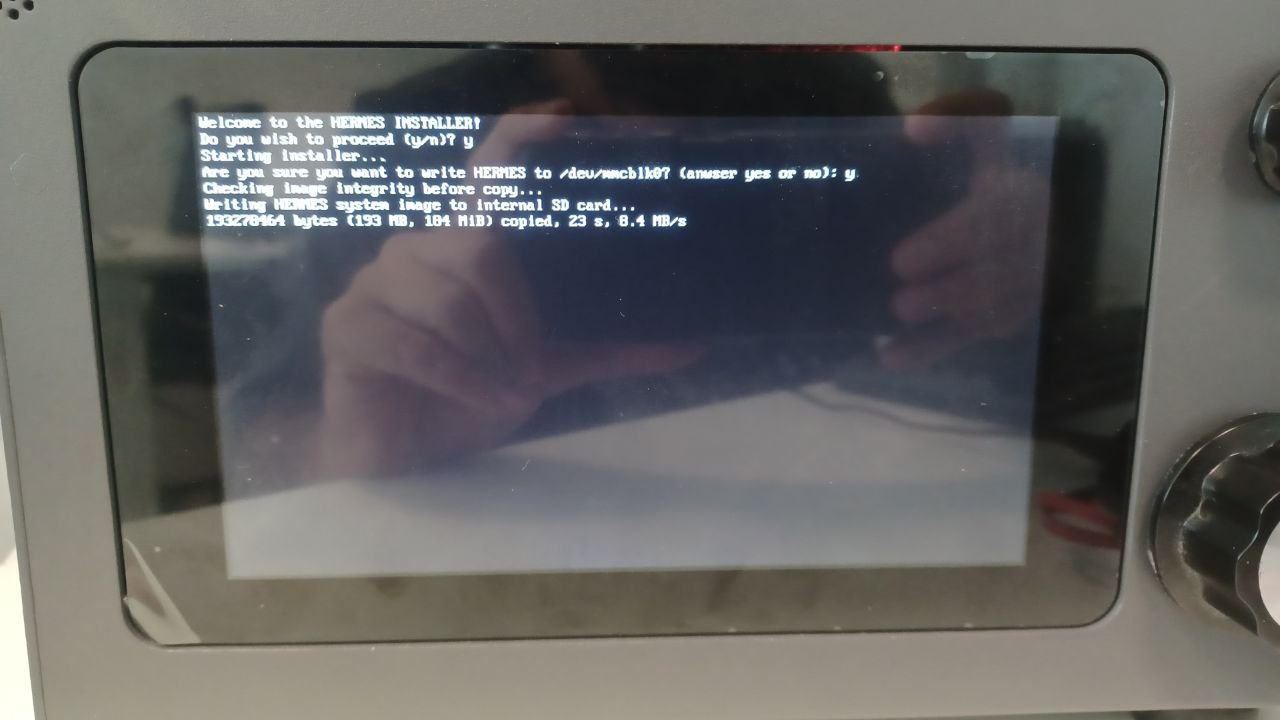
\includegraphics[width=0.5\textwidth]{pictures/inst-3.jpg}
  \caption{HERMES installer in process of copying data to internal radio memory.}
  \label{fig:inst3}
\end{figure}

After the copying is done (shown in Figure~\ref{fig:inst4}), reboot the radio (just press any key) and REMOVE the pendrive from the radio
for the second step of the installation. Also make sure the network cable (Internet) is connected to the radio.

\begin{figure}[H]
  \centering
  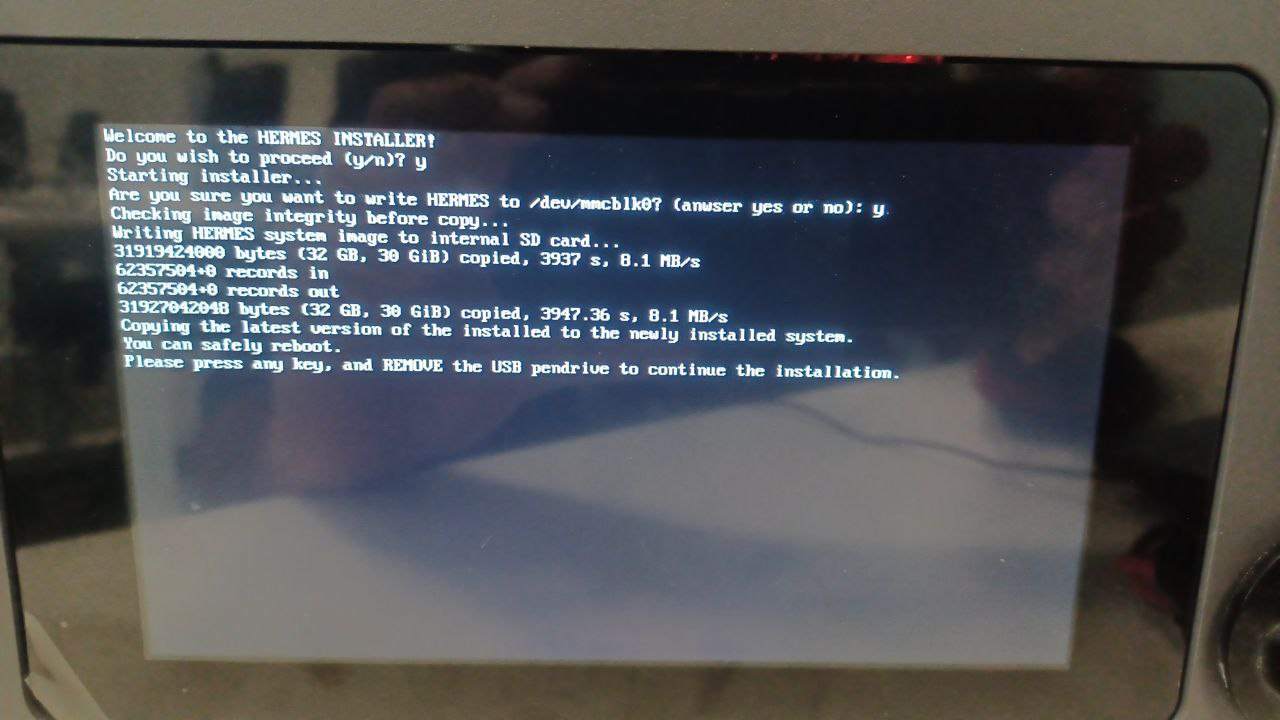
\includegraphics[width=0.5\textwidth]{pictures/inst-4.jpg}
  \caption{HERMES installer finished copy of the system to internal radio memory.}
  \label{fig:inst4}
\end{figure}


After the radio restarts, you will be asked about the station name to use, as shown in Figure~\ref{fig:inst5} and \ref{fig:inst6}. Choose one of station
names below, by typing the full station name in the installed prompt.
\begin{itemize}
\item bakouma.aco-connexion.org
\item bangassouhub.aco-connexion.org
\item briahub.aco-connexion.org
\item goboudou.aco-connexion.org
\item irabanda.aco-connexion.org
\end{itemize}

The station ``bangassouhub.aco-connexion.org'' has the gateway station setup. The gateway station should be deployed
in a place with Internet connection.

\begin{figure}[H]
  \centering
  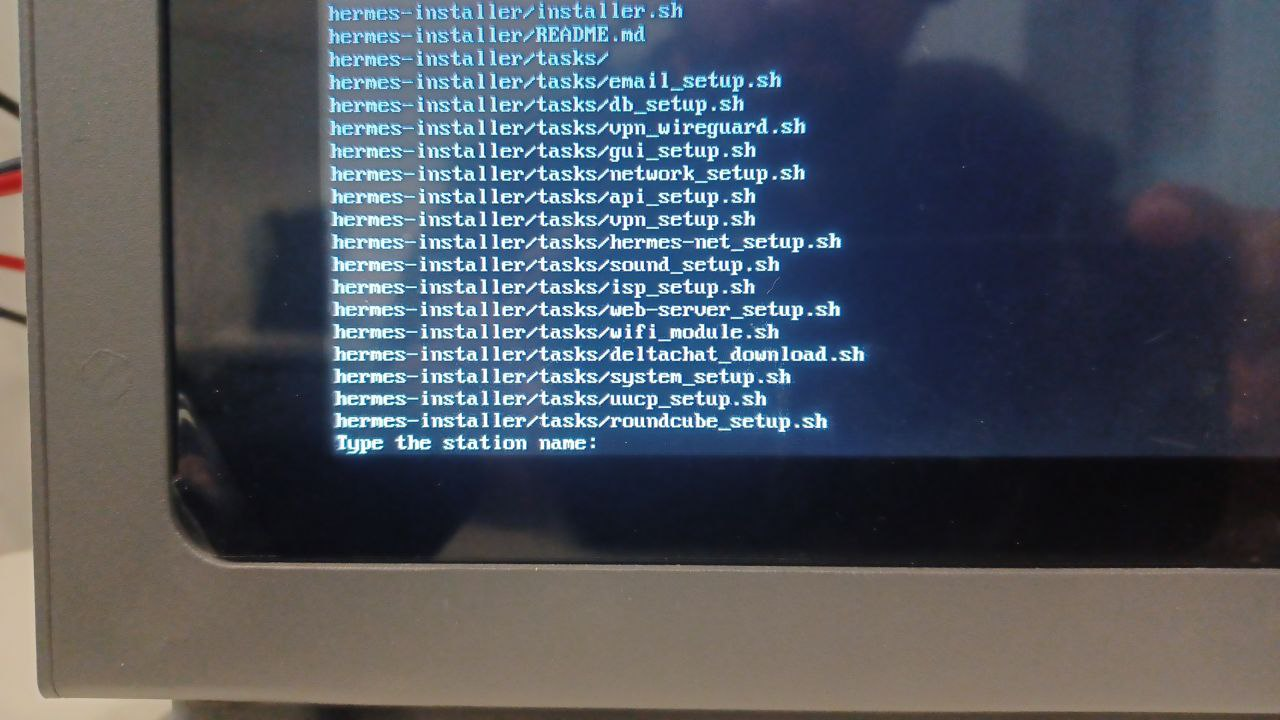
\includegraphics[width=0.5\textwidth]{pictures/inst-5.jpg}
  \caption{HERMES installer station name prompt.}.
  \label{fig:inst5}
\end{figure}

\begin{figure}[H]
  \centering
  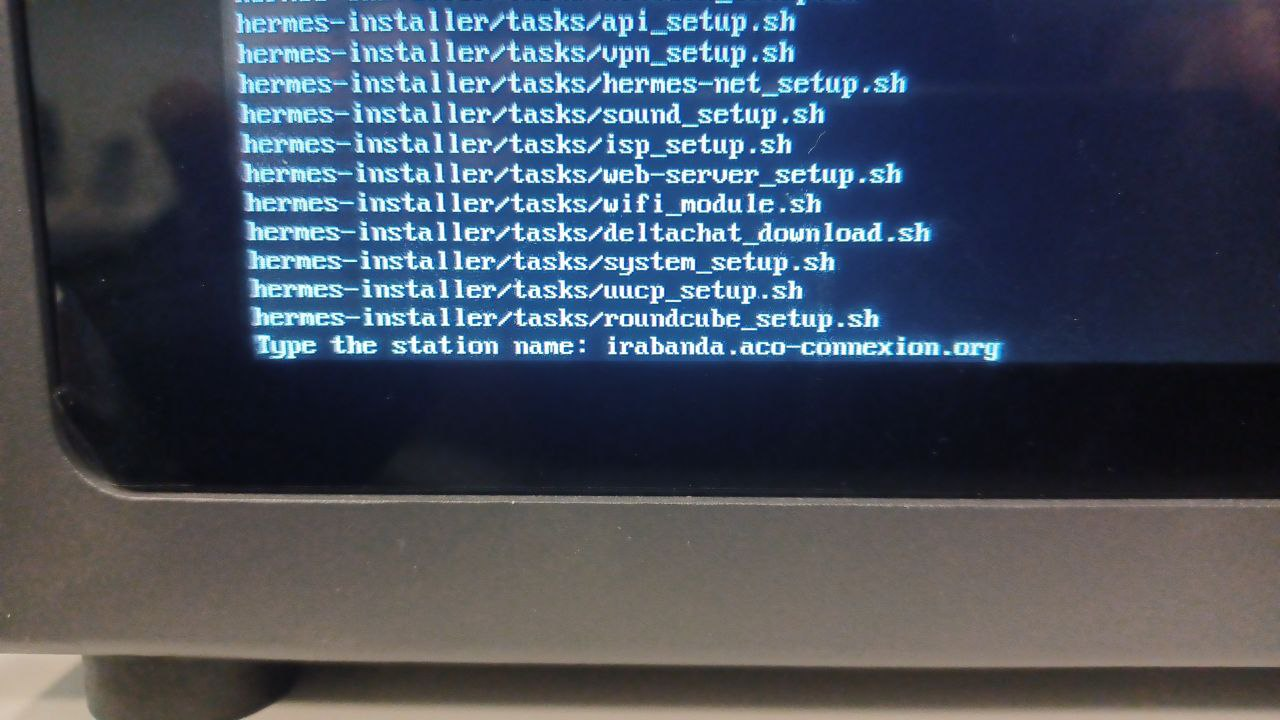
\includegraphics[width=0.5\textwidth]{pictures/inst-6.jpg}
  \caption{Station name field filled with ``irabanda.aco-connexion.org''.}.
  \label{fig:inst6}
\end{figure}

After the setup is finished, you should see the following message ``Press any key to REBOOT the radio...'', as shown in Figure~\ref{fig:inst7}. Press any key. The installation process is finished.


\begin{figure}[H]
  \centering
  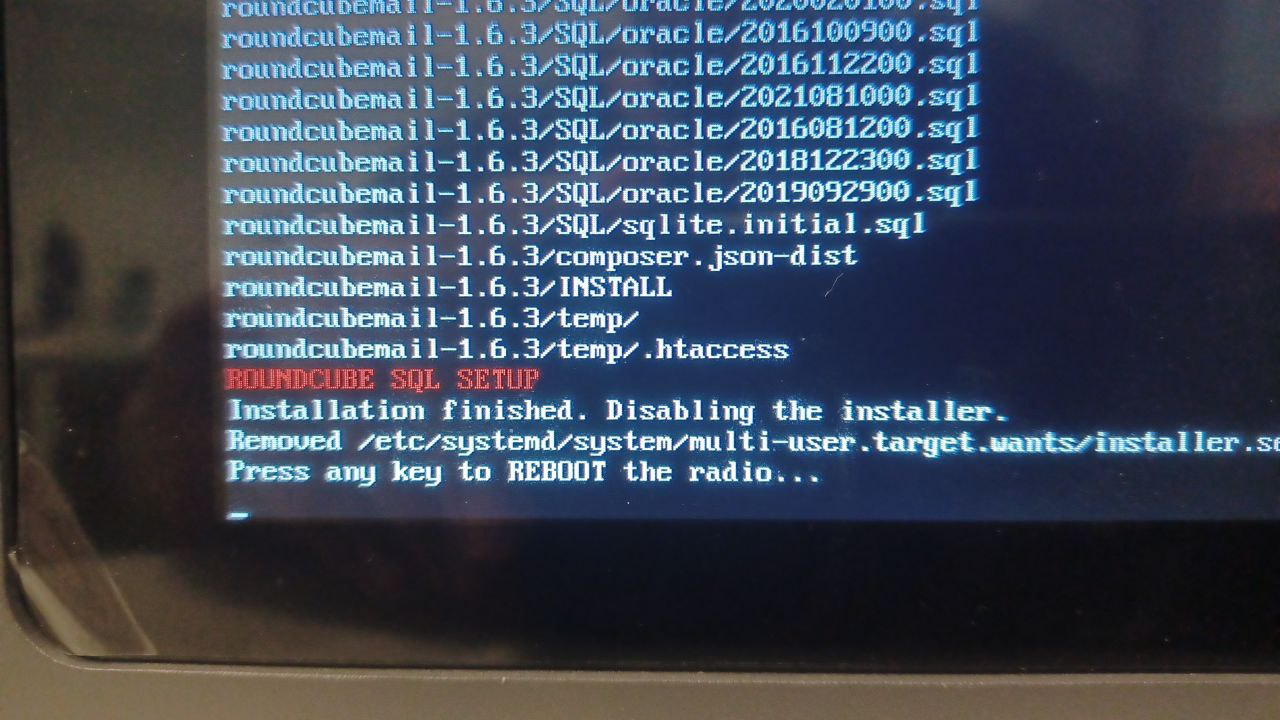
\includegraphics[width=0.5\textwidth]{pictures/inst-7.jpg}
  \caption{Message that marks the end of installation.}
  \label{fig:inst7}
\end{figure}

The radio will restart, and the HERMES interface will show up, as shown in Figure~\ref{fig:inst8}.

\begin{figure}[H]
  \centering
  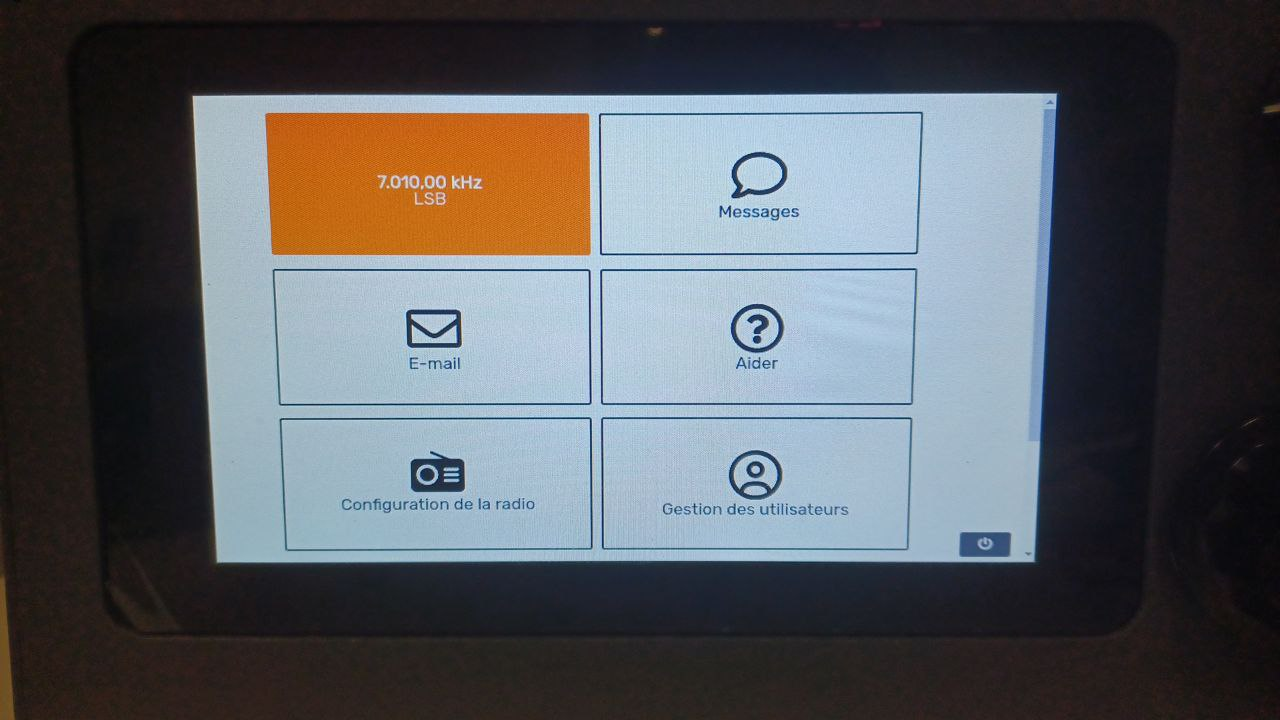
\includegraphics[width=0.5\textwidth]{pictures/inst-8.jpg}
  \caption{HERMES system screen.}
  \label{fig:inst8}
\end{figure}



% \section{WiFi}



% default password... root /


\section{Radio Frequency (RF) connections assembly}

For proper testing, the radio needs to be connected, ideally, to a power meter (also called wattmeter), which should be connected to a dummy load, as shown in Figures \ref{fig:backview1} and \ref{fig:backview3}.

\begin{figure}[H]
  \centering
  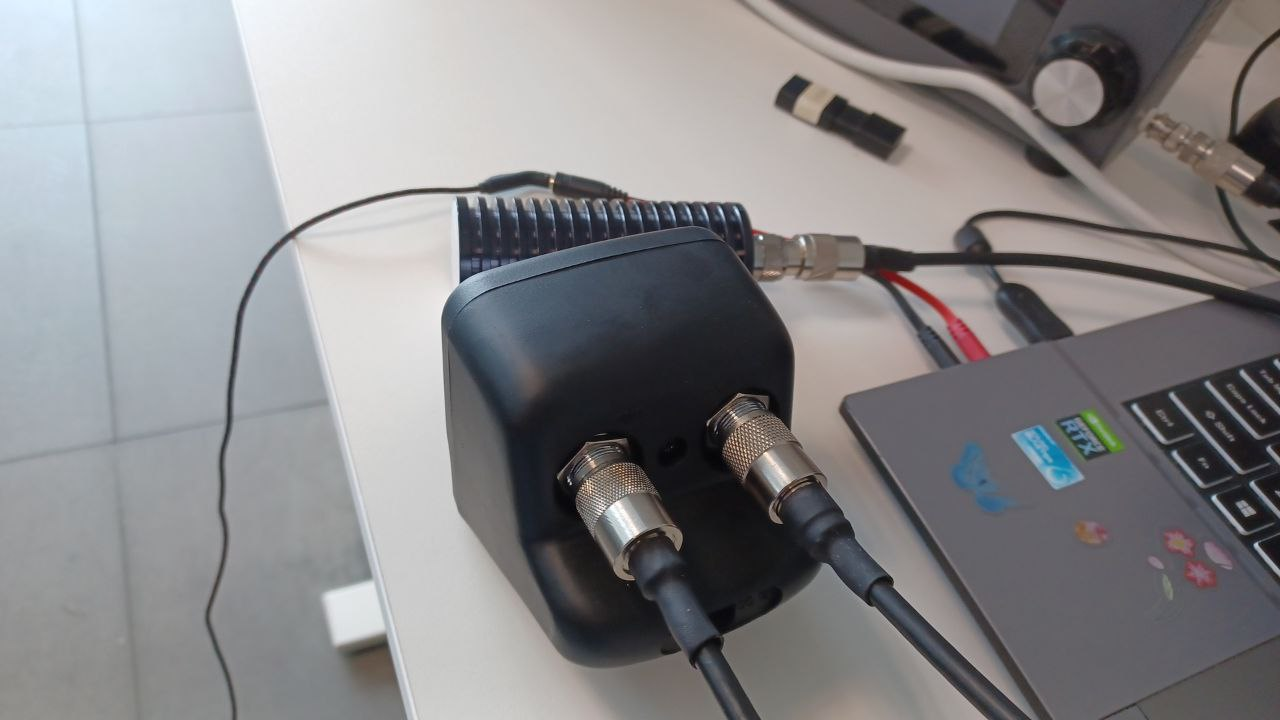
\includegraphics[width=0.5\textwidth]{pictures/wattmeter_1.jpeg}
  \caption{Back of the power meter with the cables attached.}
  \label{fig:backview1}
\end{figure}

\begin{figure}[H]
  \centering
  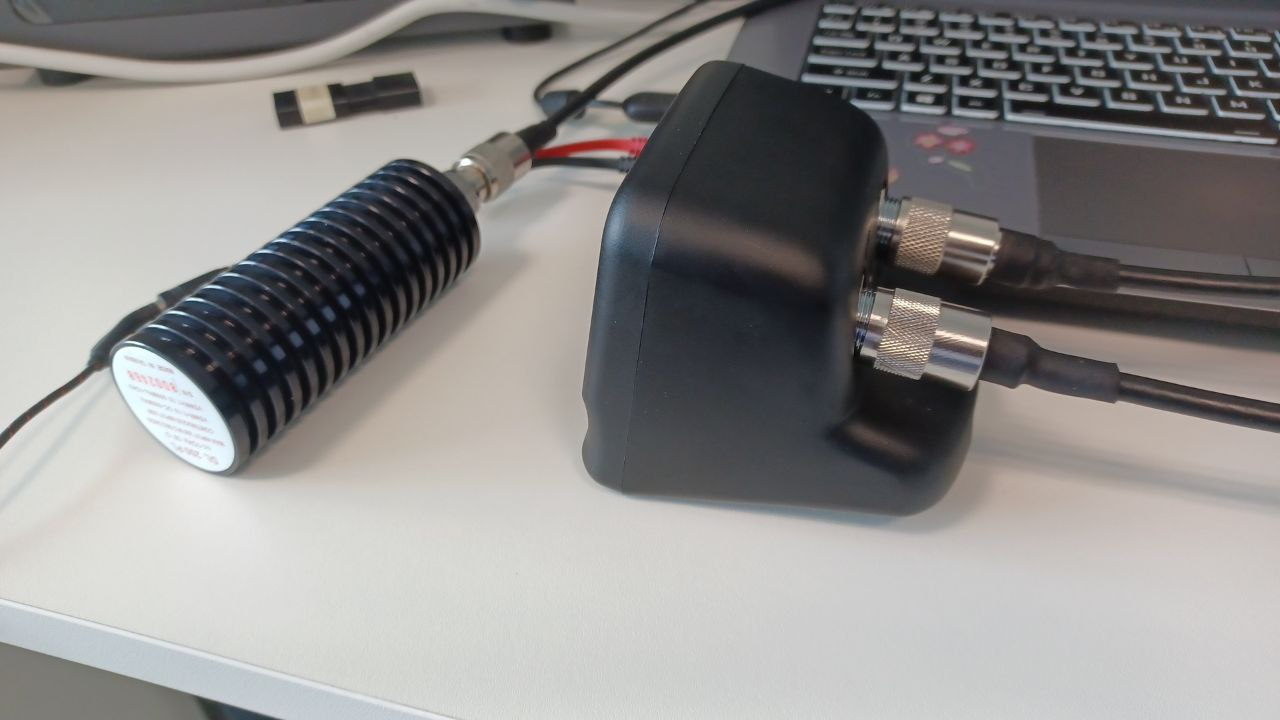
\includegraphics[width=0.5\textwidth]{pictures/wattmeter_3.jpeg}
  \caption{Both the dummy load (left) and the power meter (right).}
  \label{fig:backview3}
\end{figure}


The radio (sBitx v2) has a BNC female connector, and needs the appropriate cables and adapters to
be connected to the Wattmeter and dummy load (eg. by using BNC Male to UHF/SO239 Female). The wattmeter measures the forward and reflected power of the radio,
and the dummy load simulates an antenna without radiating the signal.

The radio needs to be connected (see Figure \ref{fig:backview4}) to the ``TX'' or ``Transmitter'' (see Figure \ref{fig:backview2}) port of the power meter, while the dummy load
should be connected to the ``ANT'' or ``Antenna'' port.

\begin{figure}[!ht]
  \centering
  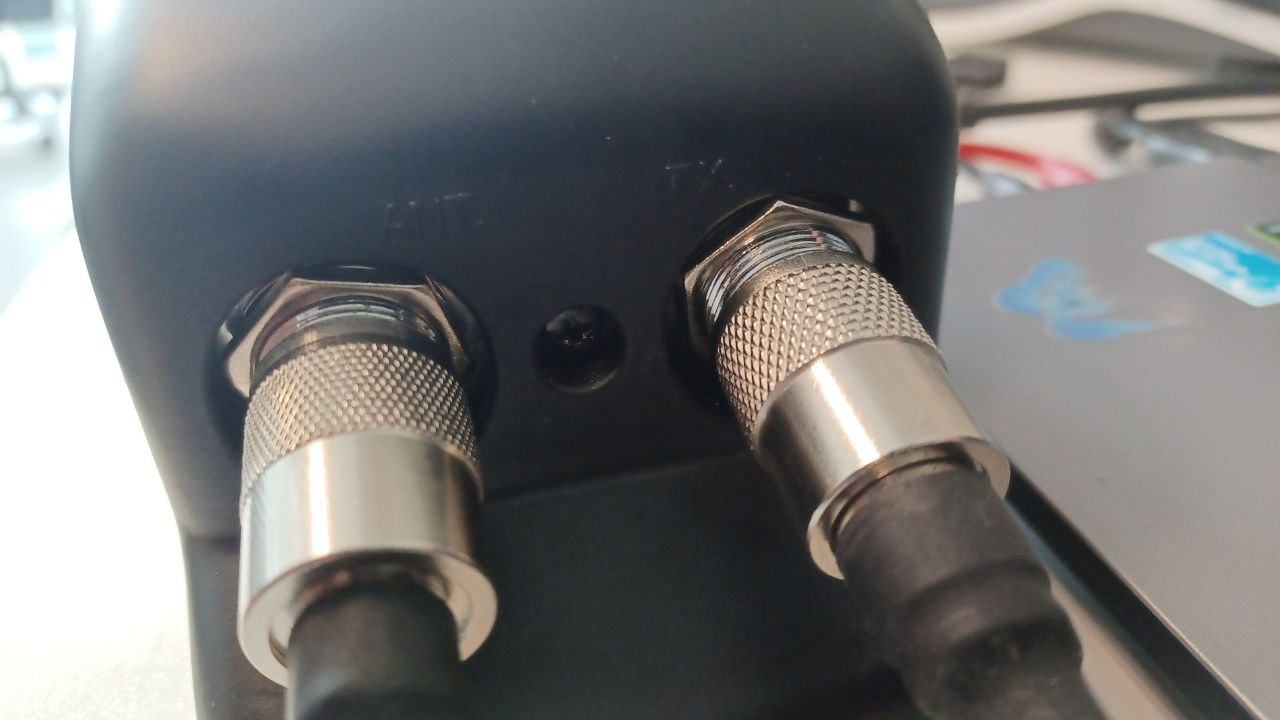
\includegraphics[width=0.7\textwidth]{pictures/wattmeter_2.jpeg}
  \caption{Back of the power meter in which the ANT and TX writings can be seen.}
  \label{fig:backview2}
\end{figure}

\begin{figure}[!ht]
  \centering
  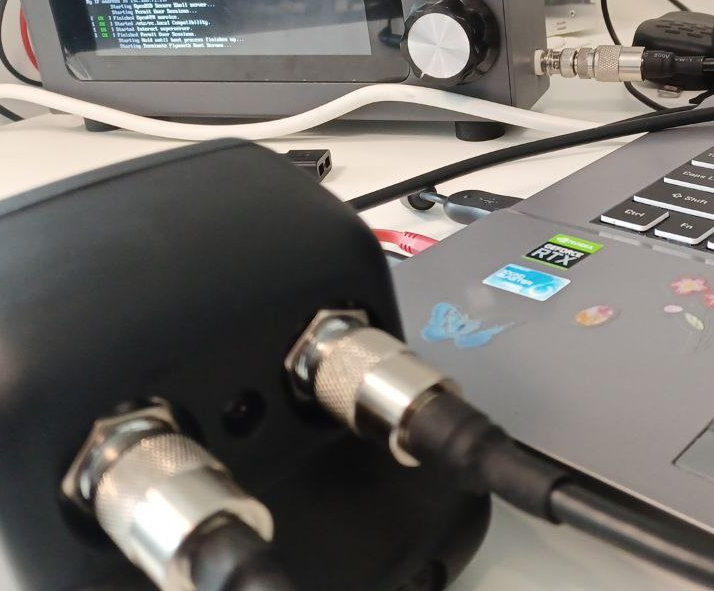
\includegraphics[width=0.5\textwidth]{pictures/wattmeter_4-edited.jpeg}
  \caption{The power meter (left) and radio with the connected cable (top right).}
  \label{fig:backview4}
\end{figure}

Make sure the cables are properly connected and the front of the power meter (Figure \ref{fig:frontview1})
is in a visible position.

\begin{figure}[!ht]
  \centering
  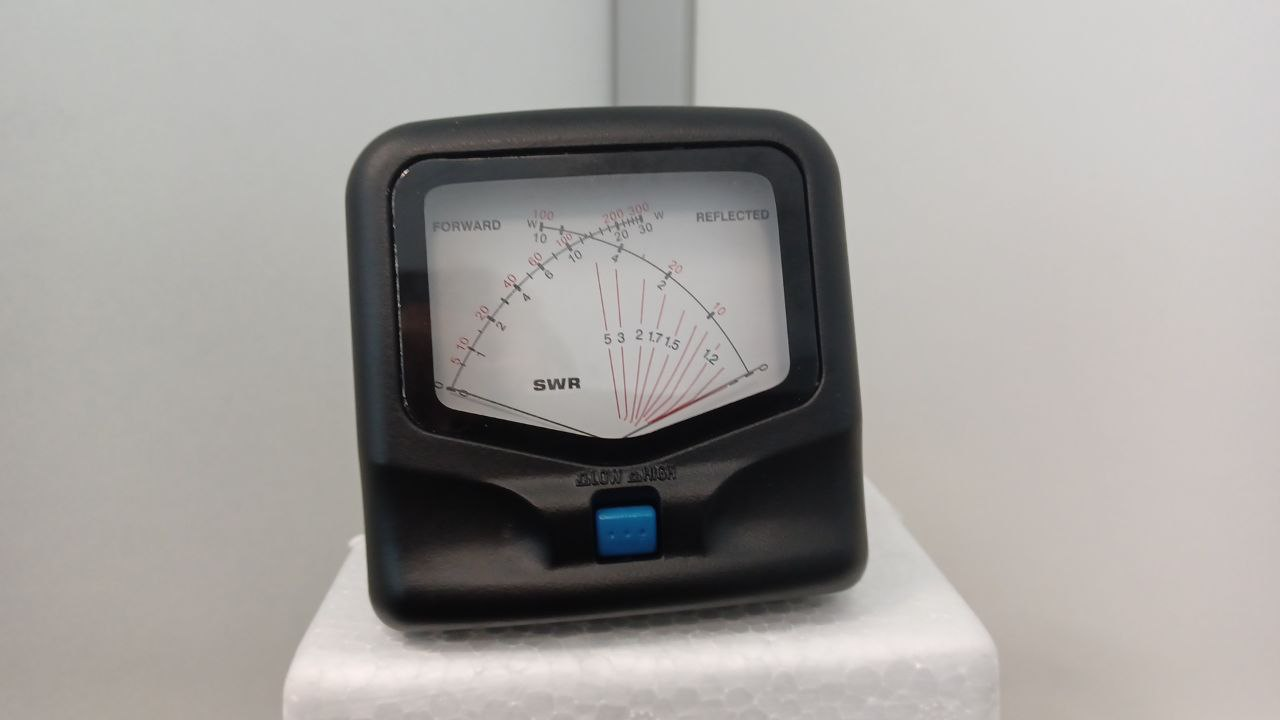
\includegraphics[width=0.5\textwidth]{pictures/wattmeter_5.jpeg}
  \caption{Front view of a power meter}
  \label{fig:frontview1}
\end{figure}

\section{RF test}
After all the RF connections ready, a transmit test needs to be made. First, set a frequency
in the band you will operate most the radio (Eg. 6200 kHz). Then two tests should be carried:
\begin{itemize}
\item Voice test with the microphone, for microphone and its button operation check
\item Single tone test, for establishing the power level of the radio
\end{itemize}

The expected result of the voice test, when talking with normal voice level, should be the wattmeter having a oscilating power level,
ranging from 0 to 40W.


% TODO: add pic of the mic/ptt

The expected result of the single tone test, should be a power reading of approximatelly 20 W.

% TODO: add pic of the single tone test

\section{WiFi Setup}
\label{sec:wifi}

Default wireless information is:
\begin{itemize}
\item Network Name (SSID): hermes
\item password: amazonia
\end{itemize}

In case the system connecting to the wifi of the radio shows a question saying that there is not internet,
questioning if you want to stay connected anyway, select the option to continue connected anyway ``always'' (in
case there is also an option to take this action ``only once'').

The Wifi settings can be changed through the HERMES interface, as shown in Figure ....

% add screenshot here...

\section{E-mail setup and test}

In this section the process of creating one or more users in the HERMES system is address. Also the process
of connecting a device (eg. tablet or cellphone) to the radio over WiFi and using the software DeltaChat (an email client)
for messages exchange.

In the HERMES interface, create one or more users, to be used for the email access. Then connect the companion
device to the radio WiFi network, and install the software DeltaChat (an email client). Follow the steps
shown in Figures ... in order to create users in the HERMES UI.

% HERMES UI screenshots...

The in the device, first connect it to the WiFi radio network, as described in section~\ref{sec:wifi}. Then open
the DeltaChat application (available in any app store, or locally in the radio, as shown in Figure ...). Use the
same login information created in the HERMES system in the DeltaChat app, and Deltachat should connect, as shown in Figures...

% DC screeshots

\end{document}
